\chapter{External Memory, Cache-Oblivious and Multi-Core Algorithms}

\section{Introduction}

\begin{figure}
\begin{center}
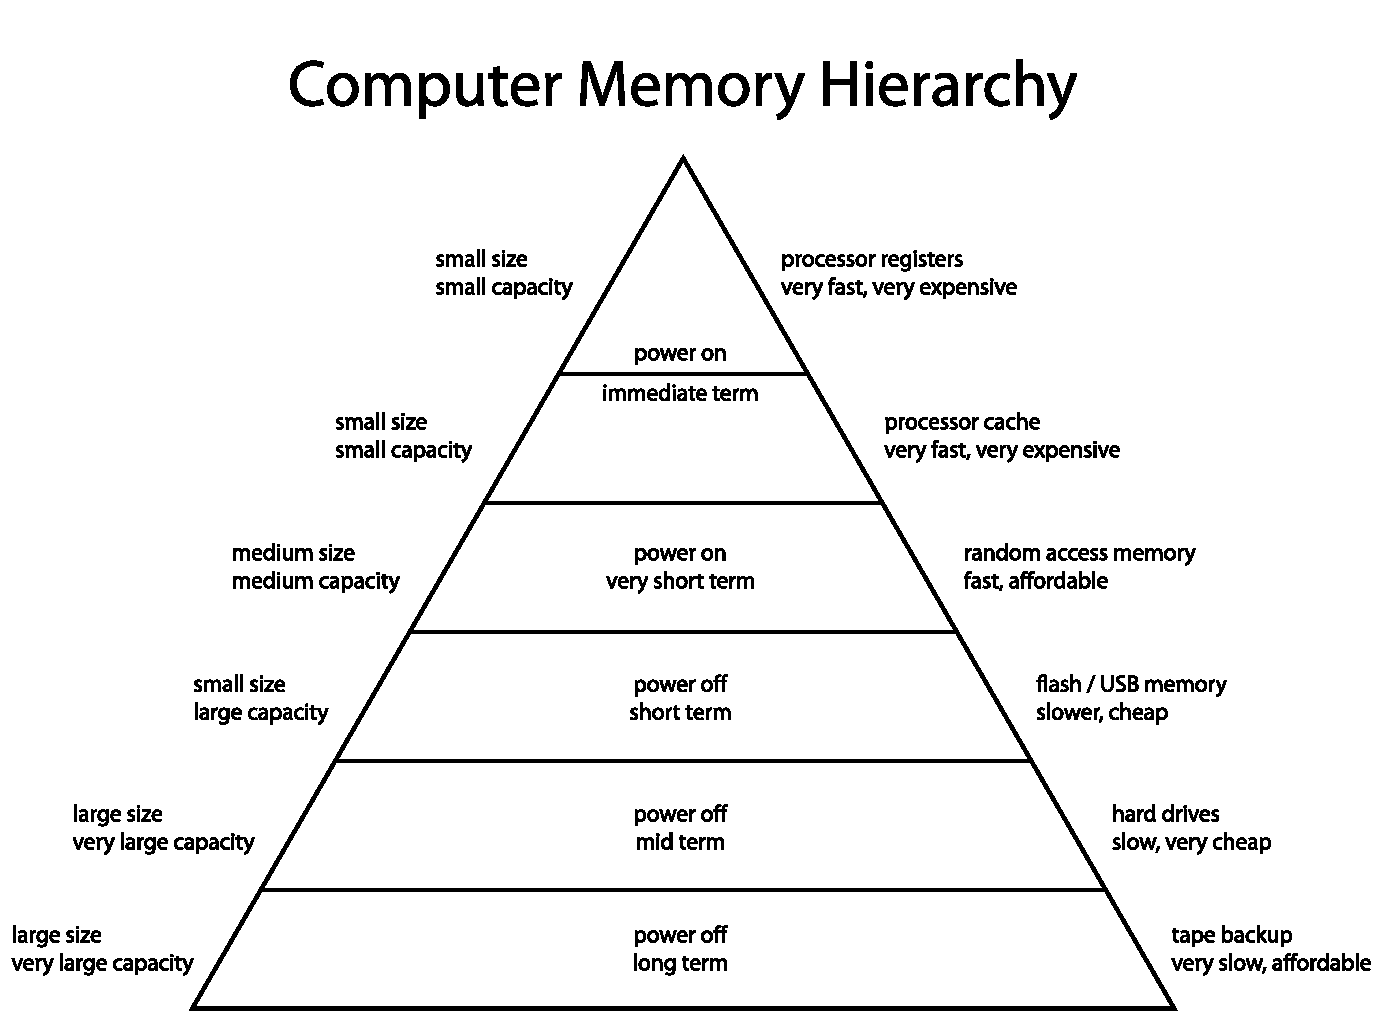
\includegraphics[width=0.8\linewidth]{./images/ComputerMemoryHierarchy}
\end{center}
\caption{Diagram showing the memory hierarchy of a modern computer architecture. From \href{http://en.wikipedia.org/wiki/File:ComputerMemoryHierarchy.svg}{Wikipedia}}
\end{figure}

CPUs run at 1 Ghz, $10^9$ instructions/sec whereas disks rotate at 6000 - 10000 rpm ( ~10 ms per rotation). Hence it takes about 10 ms until one can read the first byte from disk. The ratio of 10 ms to one cpu cycle is about $10^7$. Note that $10^7$s are roughly 100 days.

Typically the transfer rate from disk to memory is 50 MBytes/sec: in 10 ms one can move 500 kBytes. Thus in 10 ms one can read 1 Byte, in 20 ms it is possible to read 500 kBytes. This  suggests that reading data blockwise is the moste efficient access method.

\subsection{Machine model (Aggarwal/Vitter)}

When we want to optimize algorithms with respect to IO operations we use a machine model that has finite main memory of size $M$ and access to one or more disks (up to $D$). Transfers to/from disk happen in blocks of size $B$, the main memory consists of $M/B$ blocks. Up to $D$ blocks can be read or stored in parallel during one IO operation.

\section{Stack}

We want to implement an IO optimal stack. A simple method just allocates a block in main memory as a buffer. To push we write the buffer to disk if it is full and push into the buffer. Popping removes the element from the buffer if it is nonempty, else a block is read first.

This method works well for certain usage scenarios. For example $N$ pushes followed by $N$ pops require only $2 \cdot N/B$ IOs. Doing $B+1$ pushes followed by a sequence of $2$ pops, $2$ pushes, \ldots takes much more IOs: $\Omega(N)$, the worst case.

There are at least two better solutions, one of which is discussed on the exercise sheet.

The other method uses 2 blocks for the buffer.

\begin{itemize}
 \item if buffer is full, write one block to disk
 \item when buffer is empty, fetch one block from disk
\end{itemize}

After an I/O operation one block in the buffer is full, the other one empty. The next IO operation only happens after another $B$ stack operations in the worst case.

\begin{lem} The two-block solution performs $N$ stack ops with $\leq N/B$ IOs.
\end{lem}

\section{Sorting}

We know Merge Sort as an efficient sorting algorithm in main memory. It can be adapted to work with external memory too. Instead of starting with sequences of length one and merging them in pairs, we start with sequences of size $M$ (presorted in memory) and do a $k$-way merge using a binary tournament (i.e. a binary comparison tree). As the tournament requires space O($k$), we can set $k$ to be $\Theta(M/(B+O(1)))$. For simplicity assume $k=M/B$.

Generating the presorted sequences takes $2N/B$ IO operations. During each merging step the number of sequences is reduced by $k$, hence we need

\[\log_k(N/M) = \log_k(N/B)\cdot (B/M) = \log_k(N/B) - 1\]

rounds. In each round we read and write all elements, hence $2N/B$ IO operations per round.

\begin{thm} We can sort $N$ items with 

\[2\frac NB \rup{\log_{M/B} \frac NM})\]

IOs. With $D$ parallel disks, we can sort with

\[2\frac{N}{DB}\rup{\log_{M/(DB)} \frac{N}{DB}}\]

IOs.
\end{thm}